\chapter{Neural ODE and SDE}\label{sec:Neural Ordinary Differential Equation}

\glspl{neural-ode} is a class of models introduced in \cite{chen_neural_2019} : "Neural Ordinary Differential Equations" 
by Ricky T. Q. Chen, Yulia Rubanova, Jesse Bettencourt, David Duvenaud. 
ArXiV : \href{https://arxiv.org/abs/1806.07366}{Neural ODE Best Paper Award NeurIPS 2018}.\\

The starting point is to write the evolution of the latent state $z_t$ as:
\begin{align}
    z_{t+1} &= z_t + f(z_t, \theta_t)
\end{align}
where $z_t \in \mathbb{R}^D$ is the latent state, $\theta_t$ is a set
 of parameters at time $t$, and $f$ is a function.

This formulation is the one used in ResNet blocks, and can be 
seen as the Euler transformation of a continuous transformation.

Taking the expression to the limit as $dt \rightarrow 0$, we can write an 
\gls{ode}:
\begin{align}
    \frac{dz_t}{dt} &= f(z_t, t, \theta_f)
\end{align}
where $\theta_f$ is a set of parameters, that can typically be the parameters of 
a neural network learning $f$.

For a time series $x_{t_1}, x_{t_2}, ... x_{t_N}$, Chen and al. in \cite{chen_neural_2019} 
assume the following generative model:
\begin{align}
    z_{t_0} &\sim p_{\theta_z}(z_{t_0}) \\
    z_{t_1}, z_{t_2}, ..., z_{t_N} &= \text{ODE Solver}(z_{t_0}, f, \theta_f, t_0, ..., t_N ) \\
    x_{t_i} &\sim p_{\theta_x}(x_t \vert z_t)
\end{align}
We note that the latent variable is stochastic only through its initial state $z_{t_0}$. 
The evolution of $z_t$ is then deterministic through the \gls{ode}.

The inference model is:
\begin{align}
    [\mu_\phi, \Sigma_\phi] &= \text{LSTM} (x_{t_0:t_N})   \\
    q_{\phi}(z_{t_0} \vert x_{t_0:t_N}) &= \mathcal{N}(z_{t_0} \vert \mu_{\phi}, \Sigma_\phi)
\end{align}

We reproduce here the drawing from the paper:

\begin{figure}[H]
    \centering
    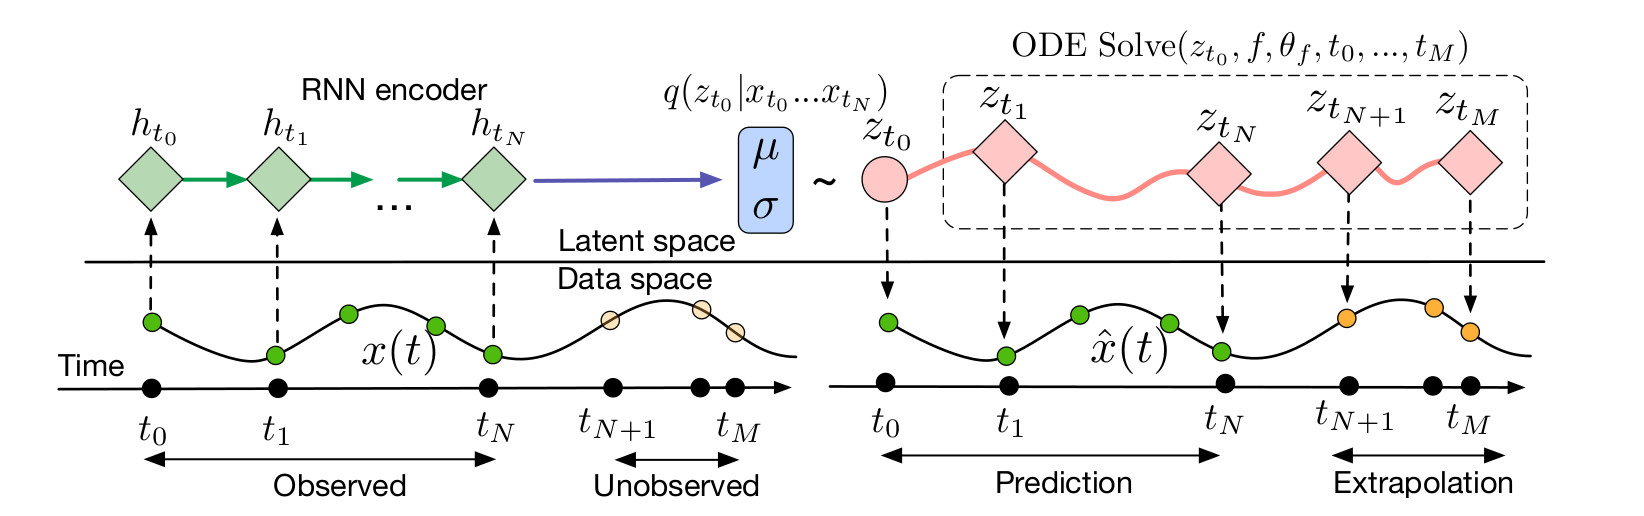
\includegraphics[width=0.9\textwidth]{/home/benjamin/Folders_Python/MVA/MVA_Stage/images/Neural_ODE_01.png}
    \caption{Neural ODE model}
    \label{fig:Neural ODE}
\end{figure}

The model is trained maximizing a \gls{vlb} as usual. 

Here, the stochastic variables are $z_{t_0}$ and the $x_{t_i}$, the joint distribution writes:
\begin{align}
    p(x_{t_1:t_N}, z_{t_0}) &= p(z_{t_0})p(x_{t_1:t_N} \vert z_{t_0}) \\
    &= p(z_{t_0}) \prod_{t=1}^{N}p_{\theta_x}(x_{t_i} \vert z_{t_i})
\end{align}
And the likelihood:
\begin{align}
    p(x_{t_1:t_N}) &= \frac{p(x_{t_1:t_N}, z_{t_0})}{p(z_{t_0} \vert x_{t_1:t_N})} \\
    \log{p(x_{t_1:t_N})} &= \mathbb{E}_{q_{\phi}(z_{t_0} \vert x_{t_1:t_N})} \log{\frac{p(x_{t_1:t_N}, z_{t_0})}{q_{\phi}(z_{t_0}\vert x_{t_1:t_N})}\frac{q_{\phi}(z_{t_0}\vert x_{t_1:t_N})}{p(z_{t_0} \vert x_{t_1:t_N})}}
\end{align}
The \gls{vlb} is:
\begin{align}
    \log{p(x_{t_1:t_N})} &\geq \mathbb{E}_{q_{\phi}(z_{t_0} \vert x_{t_1:t_N})} \log{\frac{p(x_{t_1:t_N}, z_{t_0})}{q_{\phi}(z_{t_0}\vert x_{t_1:t_N})}} \\
    &= \mathbb{E}_{q_{\phi}(z_{t_0} \vert x_{t_1:t_N})} \log{\frac{p(z_{t_0}) \prod_{t=1}^{N}p_{\theta_x}(x_{t_i} \vert z_{t_i})}{q_{\phi}(z_{t_0}\vert x_{t_1:t_N})}} \\
    &= \sum_{i=1}^{N} \mathbb{E}_{q_{\phi}(z_{t_0} \vert x_{t_1:t_N})} \log{p_{\theta_x}(x_{t_i} \vert z_{t_i})} - \mathbb{KL}(q_{\phi}(z_{t_0} \vert x_{t_1:t_N}) \vert\vert p(z_{t_0}))
\end{align}
With the simple prior $p(z_{t_0}) = \mathcal{N}(0,1)$.

Optimizing the \gls{vlb} requires that we compute the gradients on $\log{p_{\theta_x}(x_{t_i} \vert z_{t_i})}$ w.r.t. $\theta_f$, as the $z_{t_i}$ are solutions of the \gls{ode} depending 
on $f$ and its set of parameters $\theta_f$. One method is the \textbf{adjoint sensitivity method} described in \cite{pontriagin_mathematical_2018}, 
and that the interested reader will find a proof sketch in the appendix \ref{sec:adjoint_sensitivity_method}. Other methods exist, can be reviewed in \cite{sengupta_efficient_2014}.

A limitation of this model is the assumption that the prior is "concentrated" in the initial value $z_{t_0}$, and that the 
remaining latent variables are deterministically determined.

One can then modify the latent model from an \gls{ode} to a \gls{sde}:

\begin{align}
    dZ_t &= f_{\theta_f}(Z_t, t)dt + L(Z_t,t)dB_t
\end{align}

with the notations that we know well now. The adjoint sensitivity method carries over the \gls{sde}, even though I am not 
fully knowledgeable on this yet.